\section{Results}

This section presents the results of the analysis, including the performance of the optimal portfolios over 5, 7.5, and 10-year horizons. The results are visualized using various figures and tables, organized to follow the empirical specification process.

\subsection{Initial Data Analysis}

\subsubsection{Distribution of Securities by Type}
Figure \ref{fig:distribution_of_securities} shows the distribution of the securities by type.

\begin{figure}[!htbp]
    \centering
    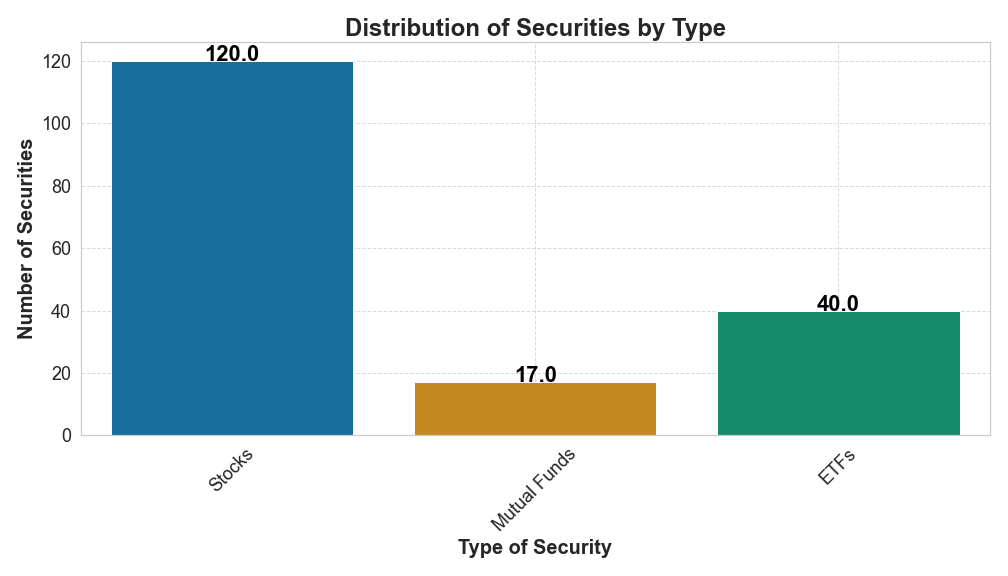
\includegraphics[width=0.8\textwidth]{../Figures/histogram_security_count.png}
    \caption{Distribution of Securities by Type}
    \label{fig:distribution_of_securities}
\end{figure}

\subsubsection{Cumulative Returns by Security Type}
Figure \ref{fig:cumulative_returns_by_type} illustrates the cumulative returns over time by security type.

\begin{figure}[!htbp]
    \centering
    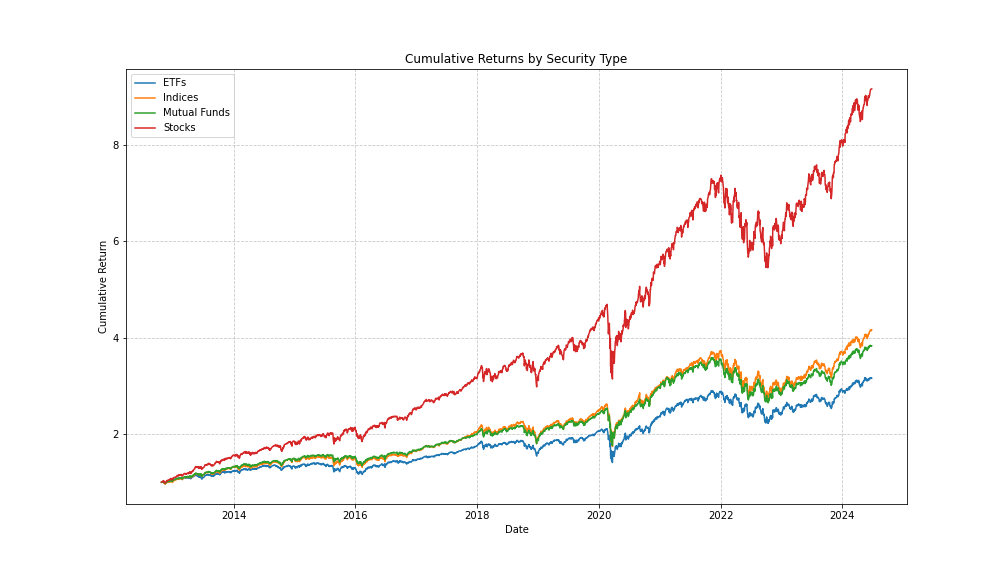
\includegraphics[width=0.8\textwidth]{../Figures/cumulative_returns_by_type.png}
    \caption{Cumulative Returns Over Time by Security Type}
    \label{fig:cumulative_returns_by_type}
\end{figure}

\textbf{Interpretation:} The majority of the securities analyzed are stocks, followed by ETFs and mutual funds. Stocks exhibit the highest cumulative return over time, indicating a higher potential for long-term growth compared to ETFs and mutual funds \citep{markowitz1952portfolio}.

\subsection{Optimal Portfolios}

\subsubsection{Top Assets by Composite Score}
Figures \ref{fig:top_assets_10y}, \ref{fig:top_assets_7_5y}, and \ref{fig:top_assets_5y} show the top assets by composite score for 10, 7.5, and 5-year horizons, respectively.

\begin{figure}[!htbp]
    \centering
    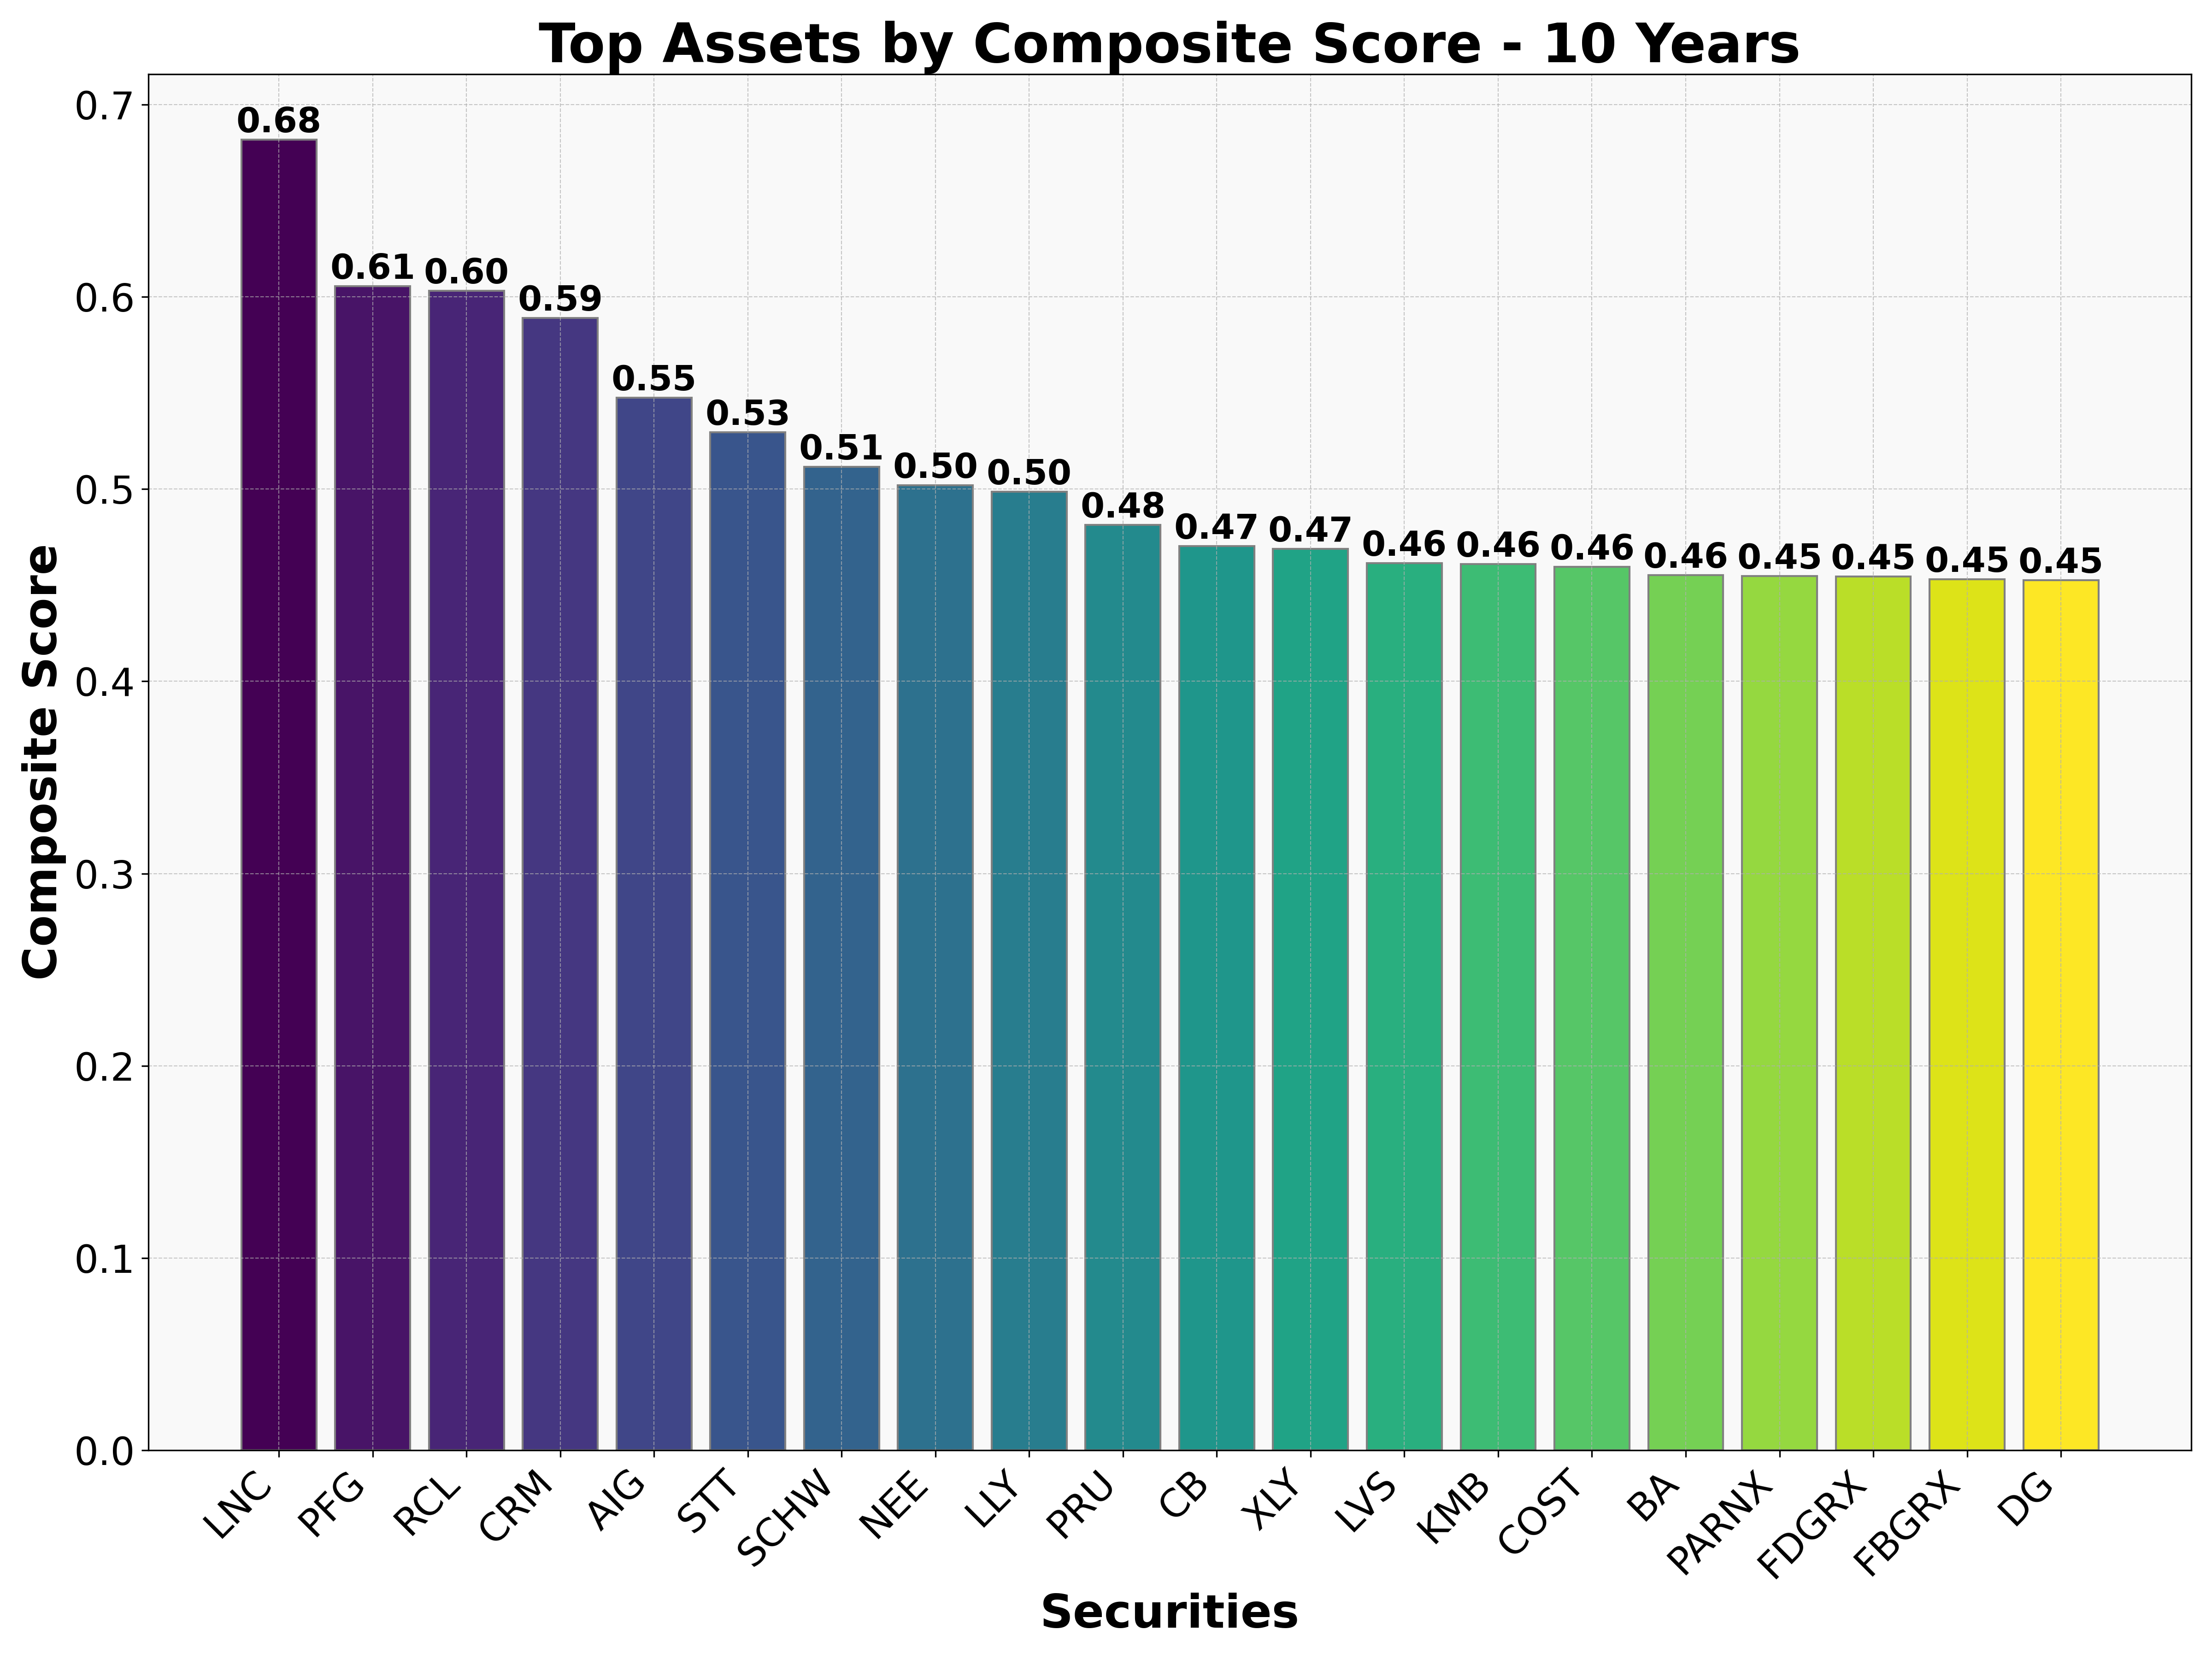
\includegraphics[width=0.8\textwidth]{../Figures/top_assets_composite_score_10_years.png}
    \caption{Top Assets by Composite Score (10 Years)}
    \label{fig:top_assets_10y}
\end{figure}

\begin{figure}[!htbp]
    \centering
    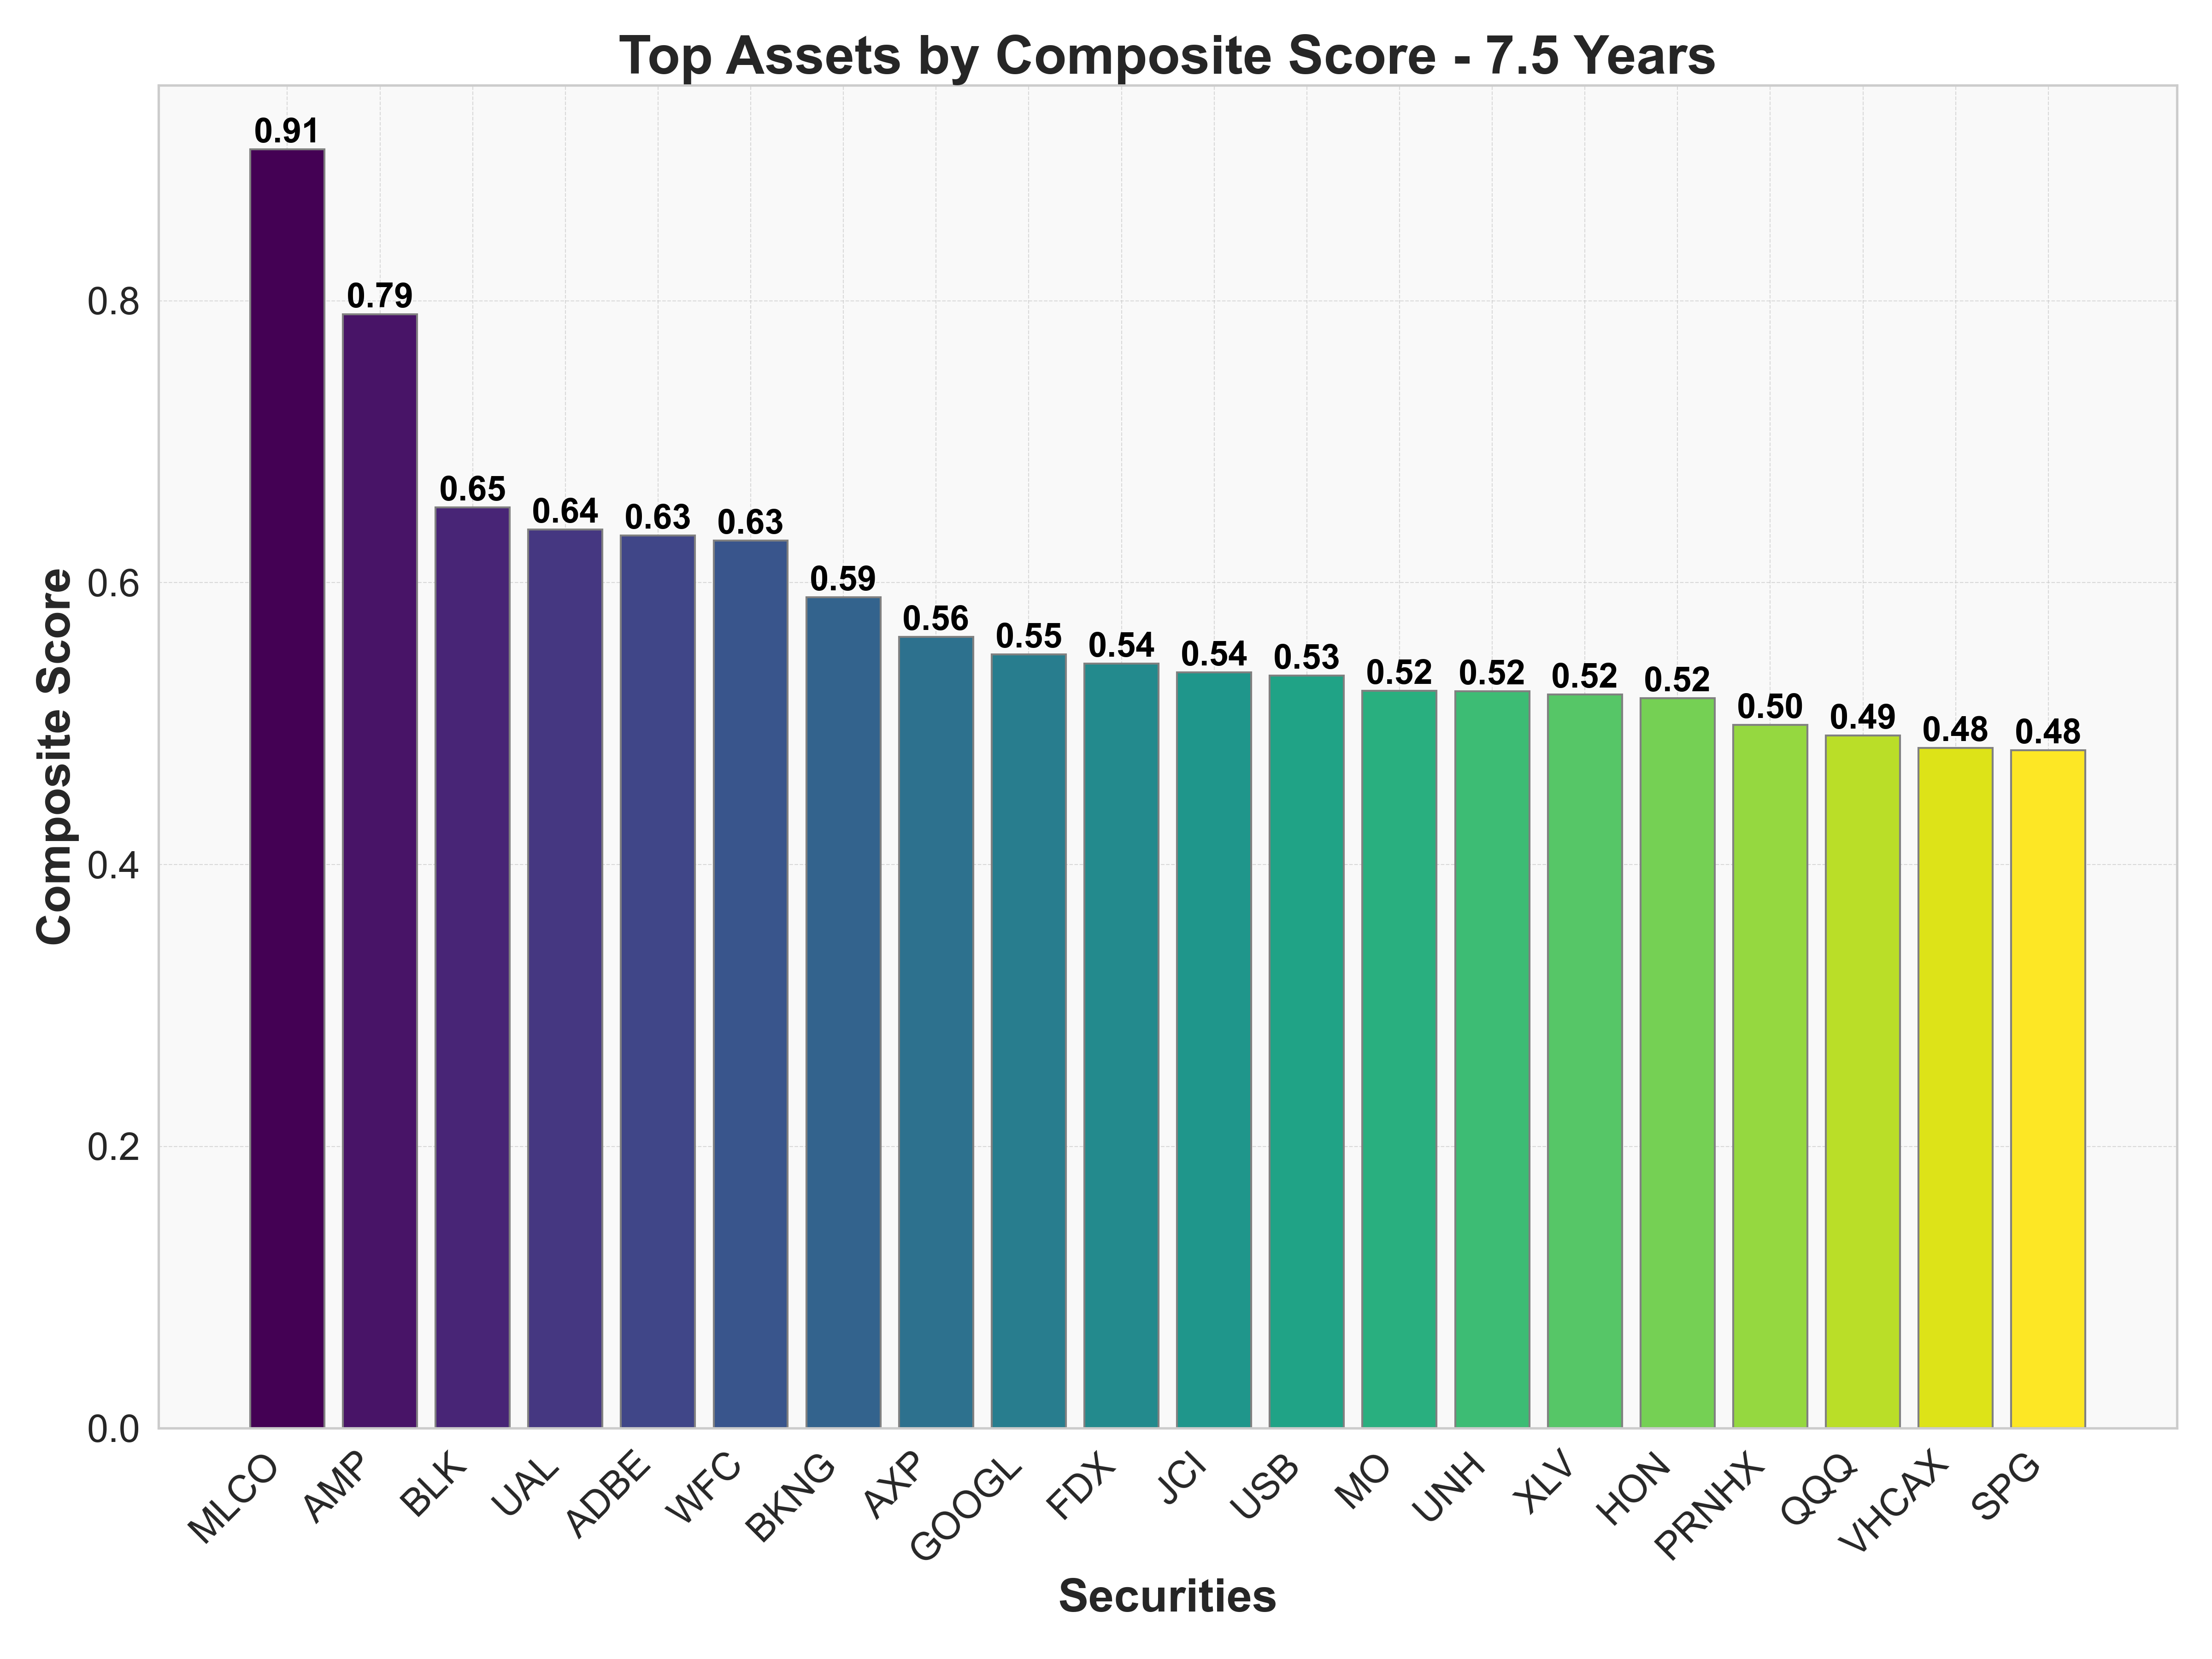
\includegraphics[width=0.8\textwidth]{../Figures/top_assets_composite_score_7_5_years.png}
    \caption{Top Assets by Composite Score (7.5 Years)}
    \label{fig:top_assets_7_5y}
\end{figure}

\begin{figure}[!htbp]
    \centering
    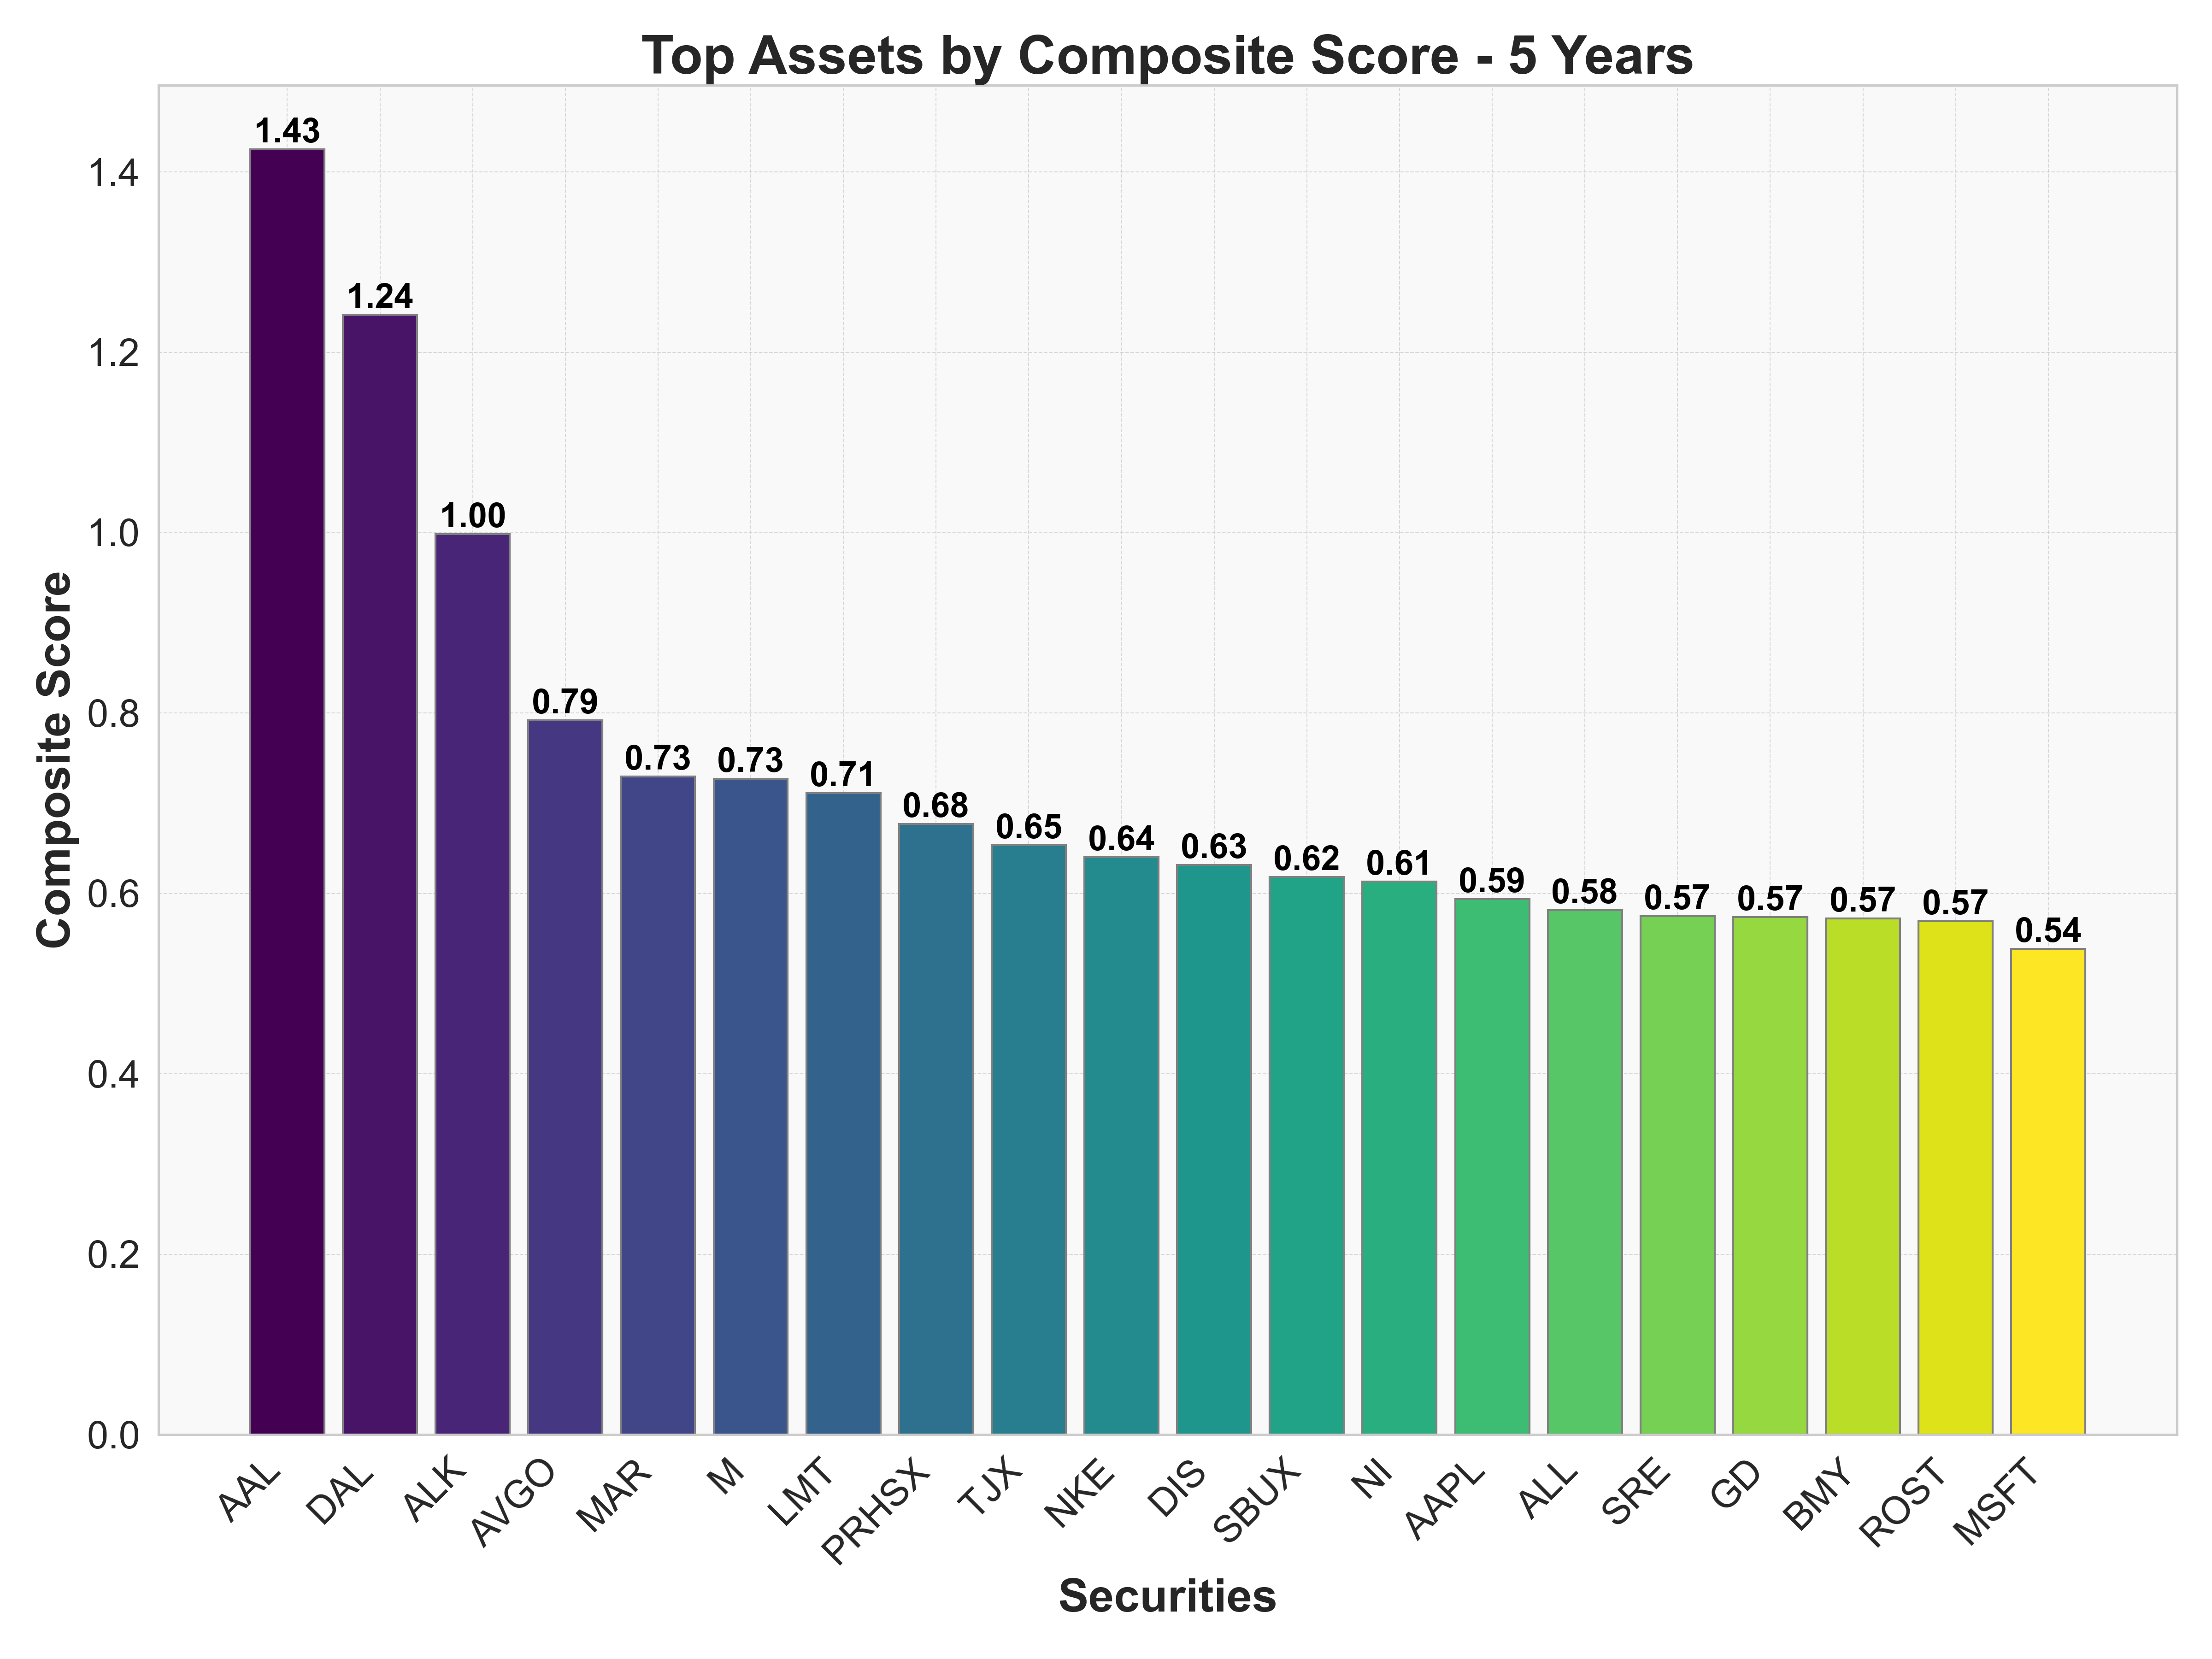
\includegraphics[width=0.8\textwidth]{../Figures/top_assets_composite_score_5_years.png}
    \caption{Top Assets by Composite Score (5 Years)}
    \label{fig:top_assets_5y}
\end{figure}

\textbf{Interpretation:} These figures highlight the top assets selected for each investment horizon based on their composite scores, indicating their suitability for different investment periods \citep{sharpe1966mutual}.

\subsubsection{Optimal Portfolios Composition}
Figures \ref{fig:optimal_portfolio_10y}, \ref{fig:optimal_portfolio_7_5y}, and \ref{fig:optimal_portfolio_5y} illustrate the composition of the optimal portfolios for 10, 7.5, and 5-year horizons, respectively.

\begin{figure}[!htbp]
    \centering
    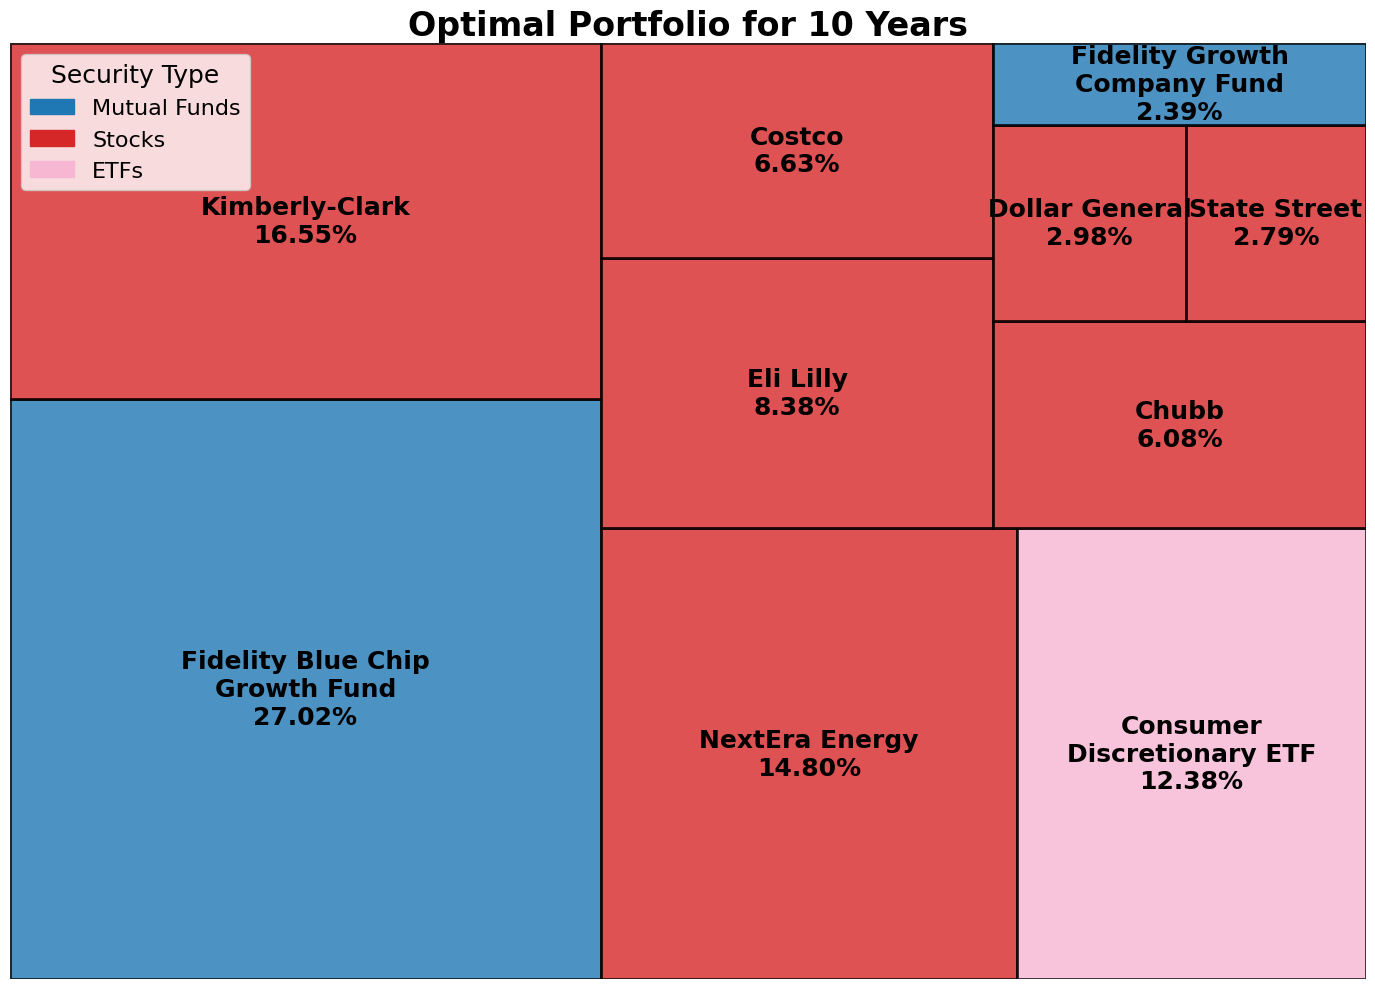
\includegraphics[width=0.8\textwidth]{../Figures/optimal_portfolio_10_years.png}
    \caption{Optimal Portfolio for 10 Years}
    \label{fig:optimal_portfolio_10y}
\end{figure}

\begin{figure}[!htbp]
    \centering
    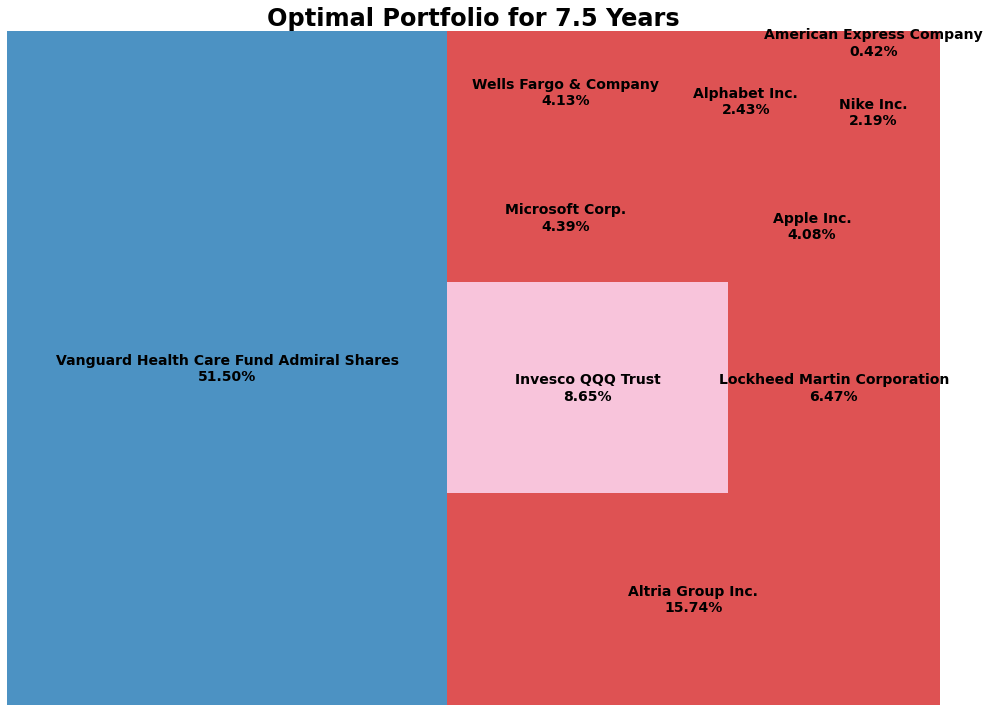
\includegraphics[width=0.8\textwidth]{../Figures/optimal_portfolio_7_5_years.png}
    \caption{Optimal Portfolio for 7.5 Years}
    \label{fig:optimal_portfolio_7_5y}
\end{figure}

\begin{figure}[!htbp]
    \centering
    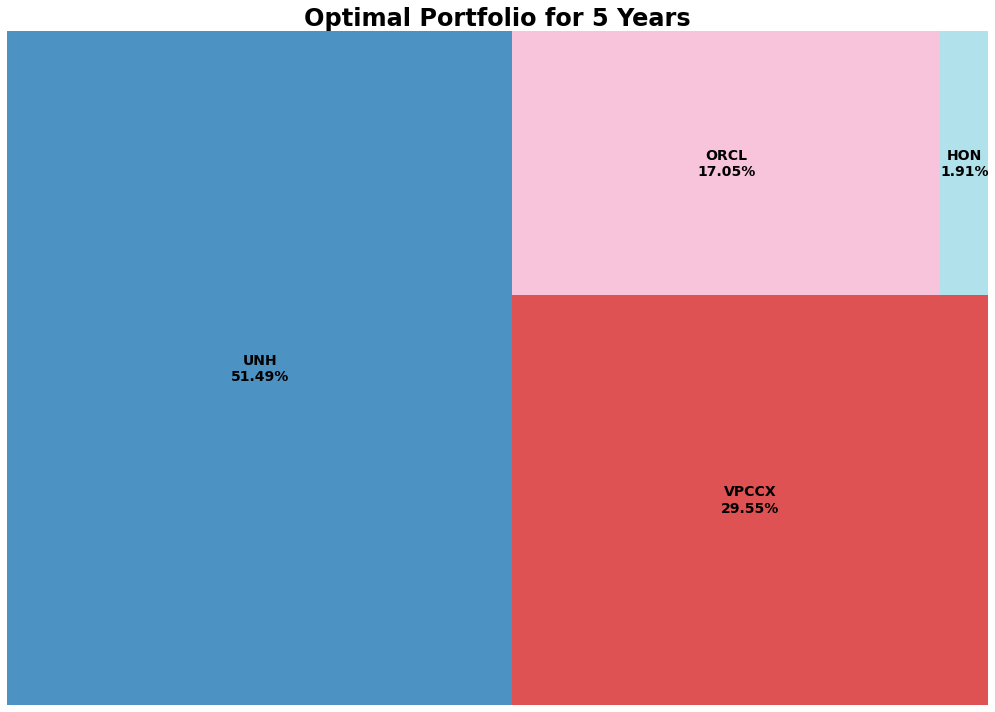
\includegraphics[width=0.8\textwidth]{../Figures/optimal_portfolio_5_years.png}
    \caption{Optimal Portfolio for 5 Years}
    \label{fig:optimal_portfolio_5y}
\end{figure}

\textbf{Interpretation:} These figures show the composition of the optimal portfolios, emphasizing long-term growth for the 10-year horizon, balanced growth and risk for the 7.5-year horizon, and more conservative assets for the 5-year horizon.

\subsection{Comparison with Hindsight Data}

\subsubsection{Cumulative Returns Comparison}
Figure \ref{fig:cumulative_returns_comparison} compares the cumulative returns of actual portfolios against the S\&P 500 benchmark.

\begin{figure}[!htbp]
    \centering
    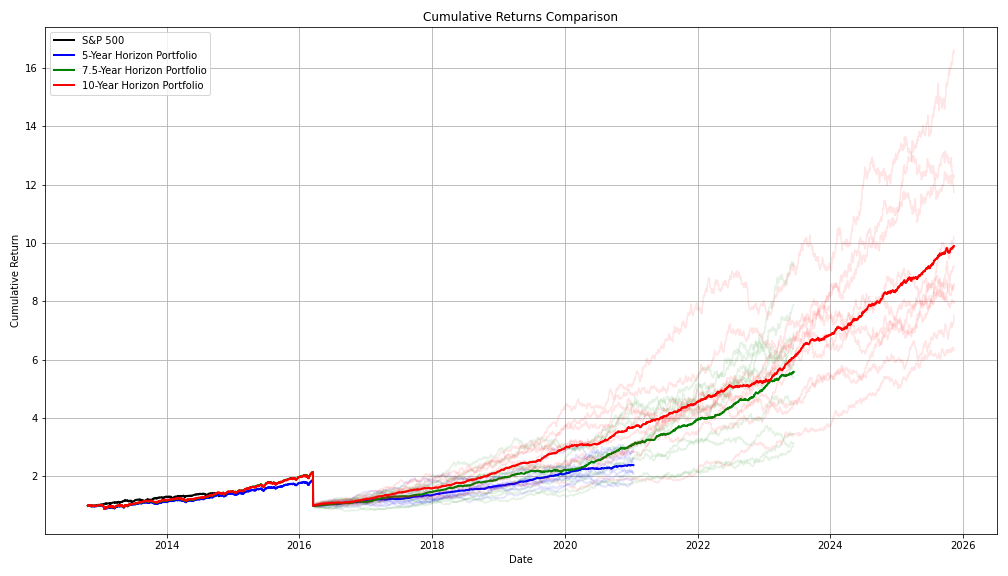
\includegraphics[width=0.8\textwidth]{../Figures/cumulative_returns_comparison.png}
    \caption{Cumulative Returns Comparison of Actual Portfolios vs. S\&P 500}
    \label{fig:cumulative_returns_comparison}
\end{figure}

\subsubsection{Cumulative Returns Summary}
Figure \ref{fig:cumulative_returns_summary} summarizes the cumulative returns for the actual portfolios over the investment horizons compared to the S\&P 500.

\begin{figure}[!htbp]
    \centering
    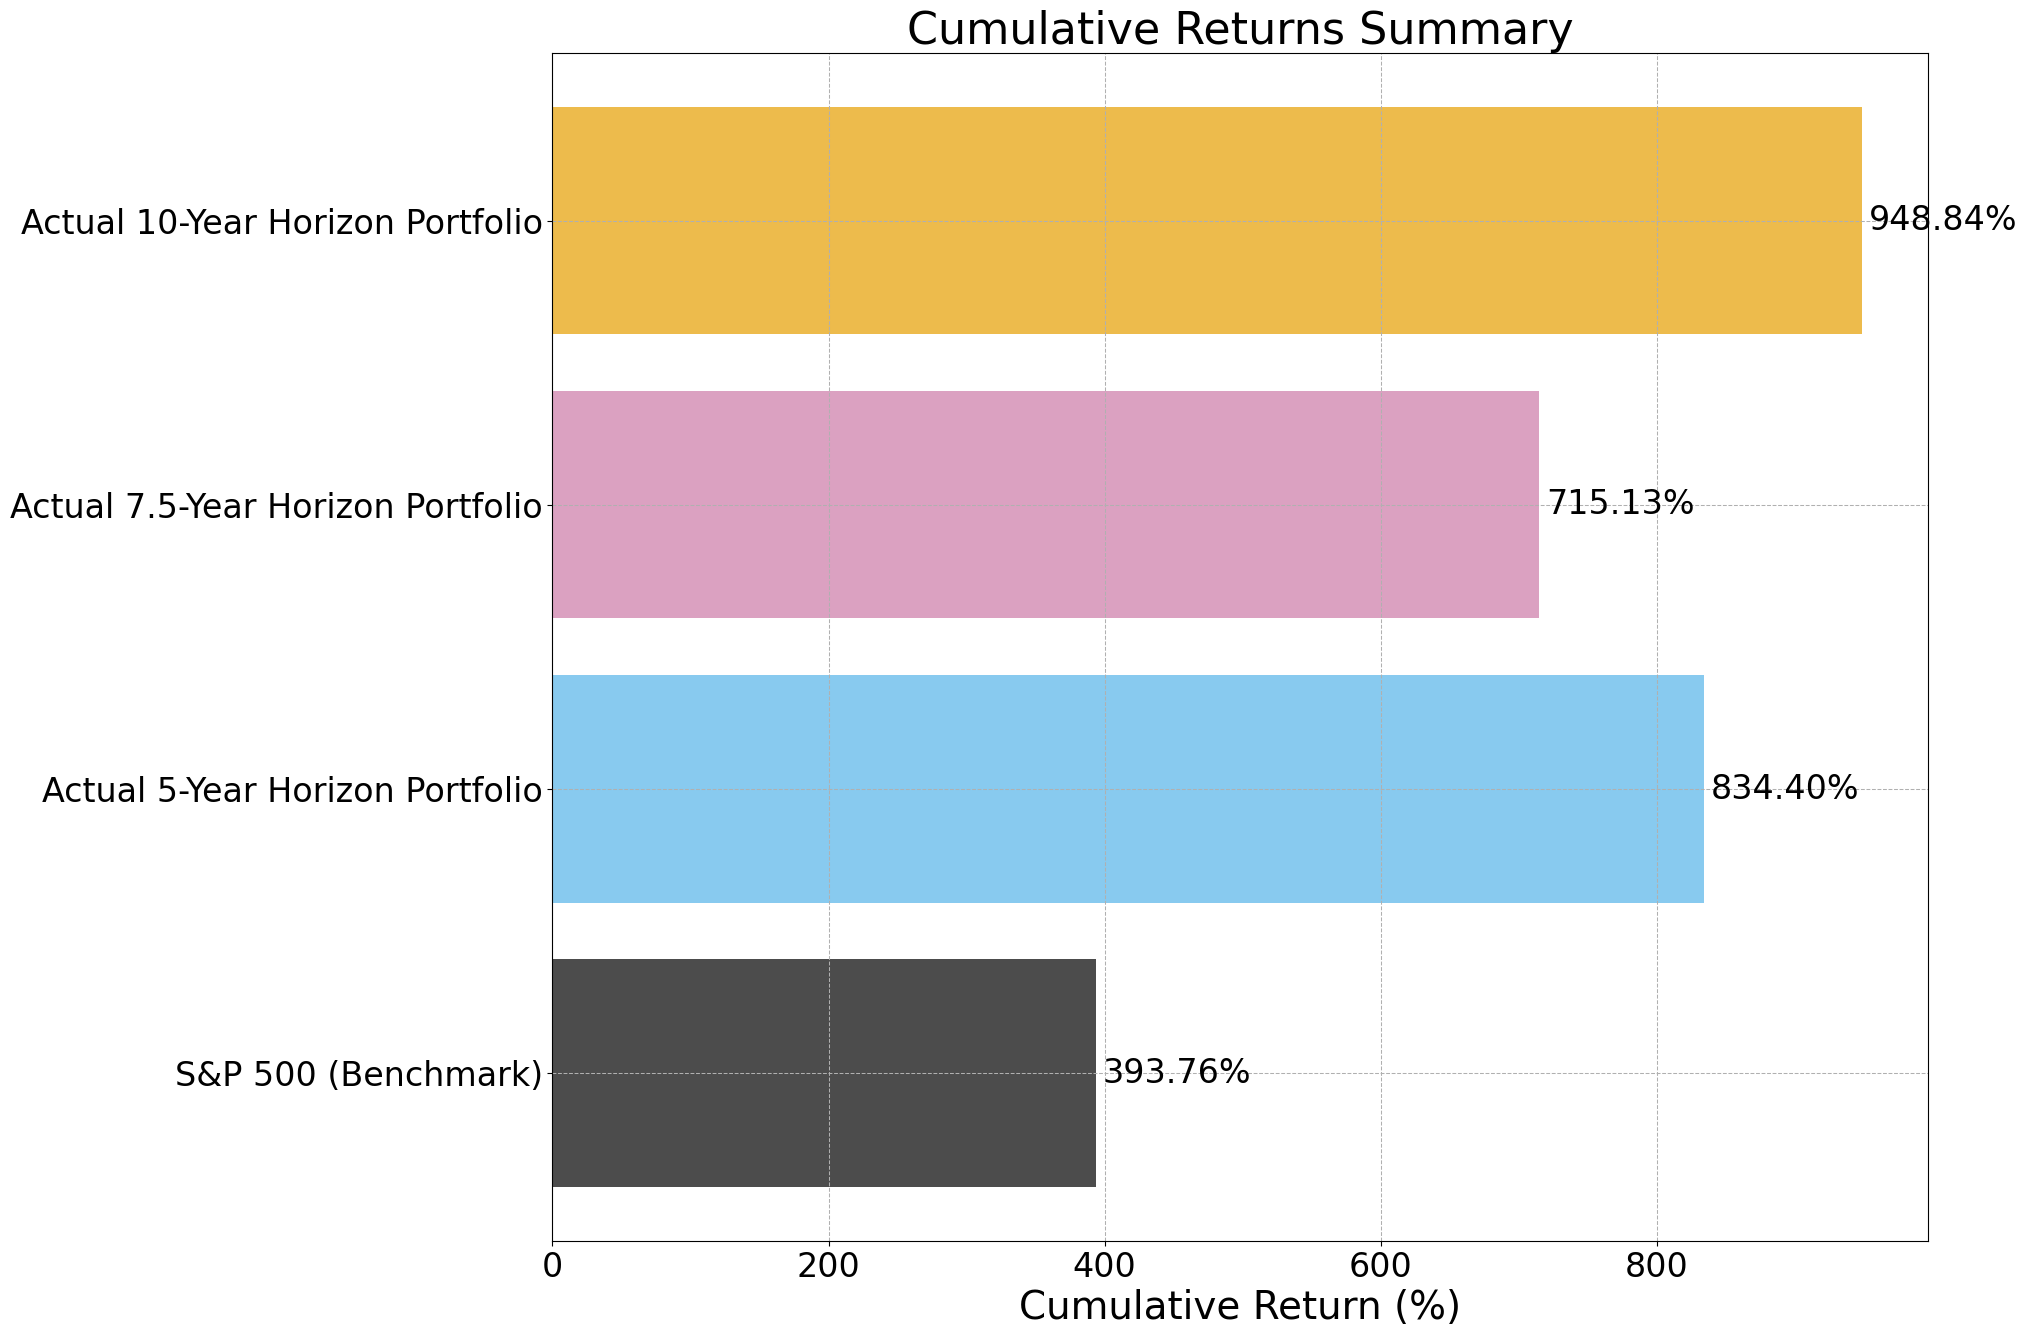
\includegraphics[width=0.8\textwidth]{../Figures/cumulative_returns_summary.png}
    \caption{Cumulative Returns Summary 2011-05-04 to 2024-07-10}
    \label{fig:cumulative_returns_summary}
\end{figure}

\textbf{Interpretation:} The optimized portfolios consistently outperform the S\&P 500 benchmark, demonstrating the effectiveness of the optimization strategy \citep{sharpe1966mutual}. The 10-year horizon portfolio exhibits the highest cumulative return, followed by the 7.5-year and 5-year horizons. These results highlight the advantage of long-term investing \citep{fama1970efficient}.

\subsection{Monte Carlo Simulation for Future Forecasting}

\subsubsection{Distribution of Final Portfolio Values}
Figures \ref{fig:final_portfolio_values_5y}, \ref{fig:final_portfolio_values_7_5y}, and \ref{fig:final_portfolio_values_10y} illustrate the distribution of final portfolio values for 5, 7.5, and 10-year investment horizons, respectively.

\begin{figure}[!htbp]
    \centering
    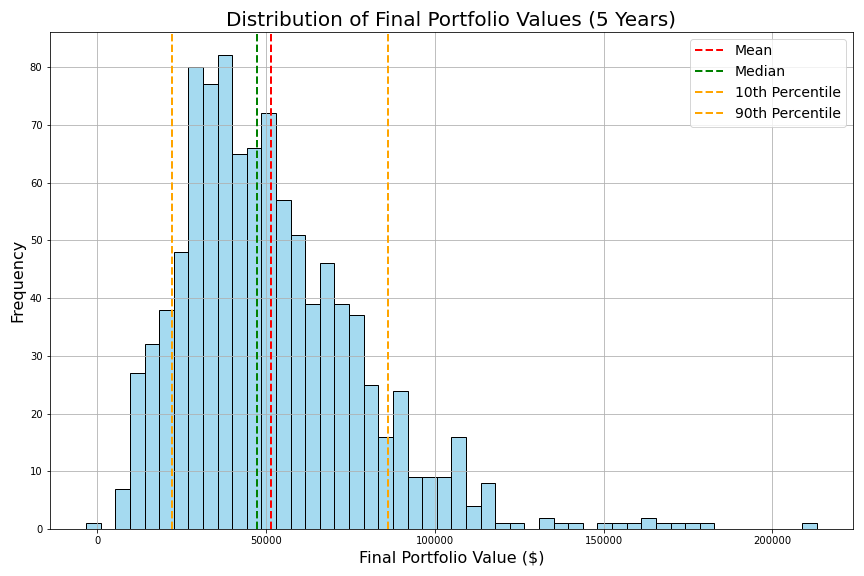
\includegraphics[width=0.8\textwidth]{../Figures/final_portfolio_values_distribution_5_years.png}
    \caption{Distribution of Final Portfolio Values (5 Years)}
    \label{fig:final_portfolio_values_5y}
\end{figure}

\begin{figure}[!htbp]
    \centering
    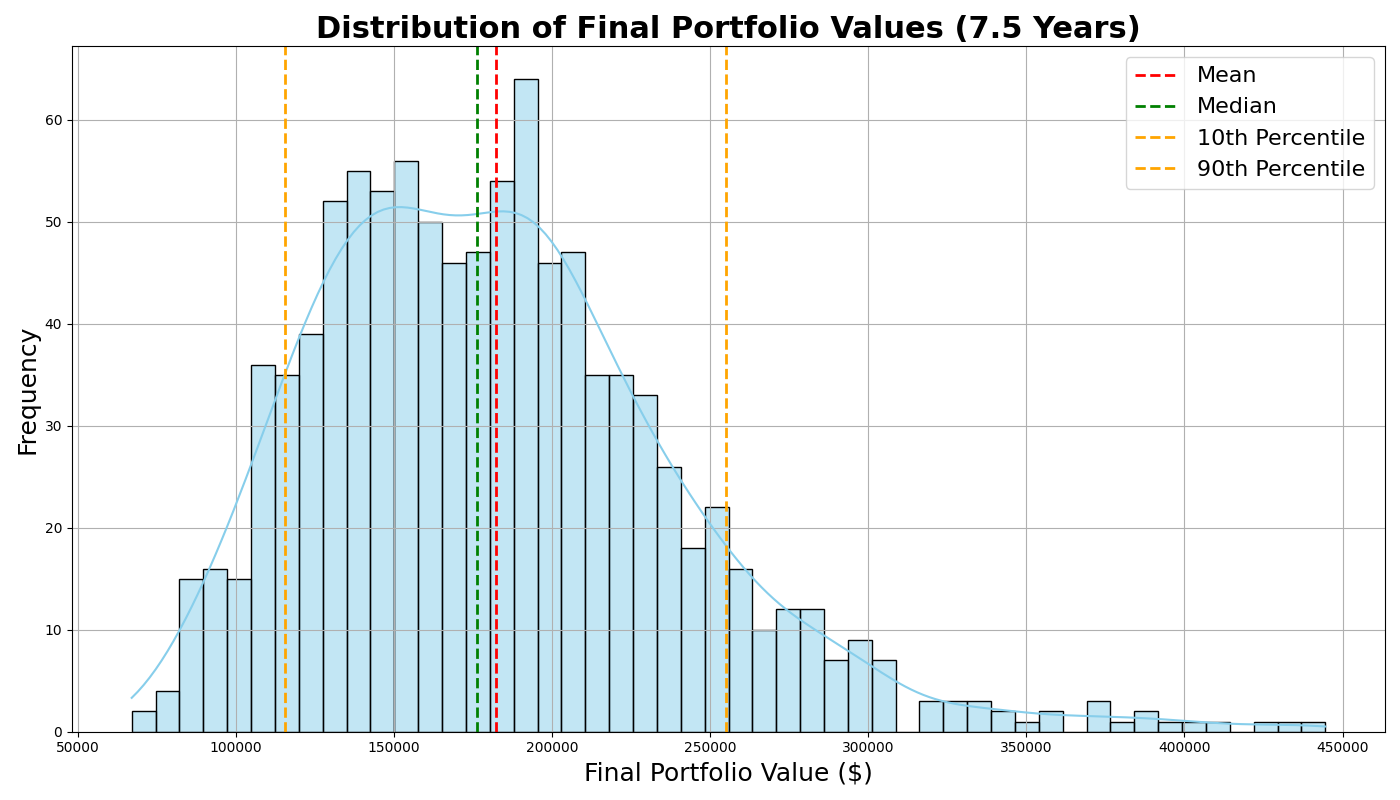
\includegraphics[width=0.8\textwidth]{../Figures/final_portfolio_values_distribution_7_5_years.png}
    \caption{Distribution of Final Portfolio Values (7.5 Years)}
    \label{fig:final_portfolio_values_7_5y}
\end{figure}

\begin{figure}[!htbp]
    \centering
    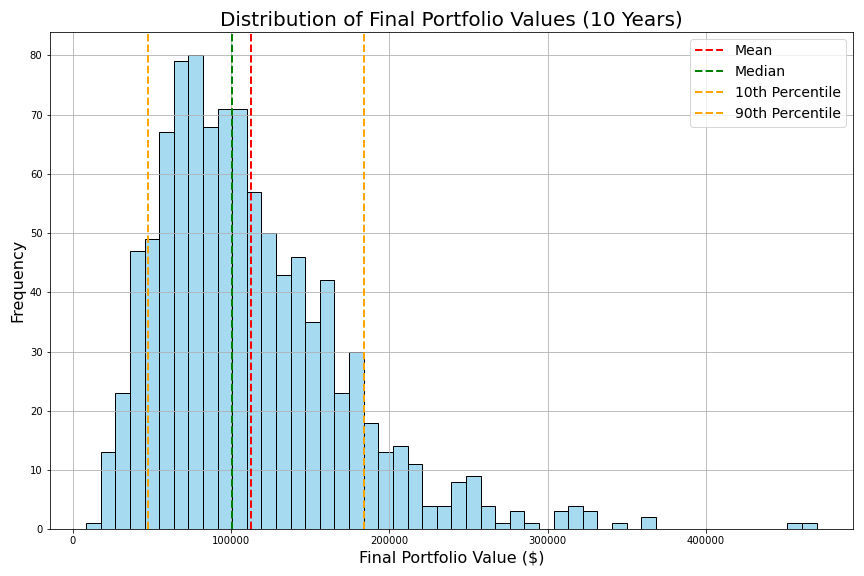
\includegraphics[width=0.8\textwidth]{../Figures/final_portfolio_values_distribution_10_years.png}
    \caption{Distribution of Final Portfolio Values (10 Years)}
    \label{fig:final_portfolio_values_10y}
\end{figure}

\subsubsection{Cumulative Returns Over Time}
Figures \ref{fig:cumulative_returns_5y}, \ref{fig:cumulative_returns_7_5y}, and \ref{fig:cumulative_returns_10y} show the cumulative returns over time for 5, 7.5, and 10-year investment horizons, respectively.

\begin{figure}[!htbp]
    \centering
    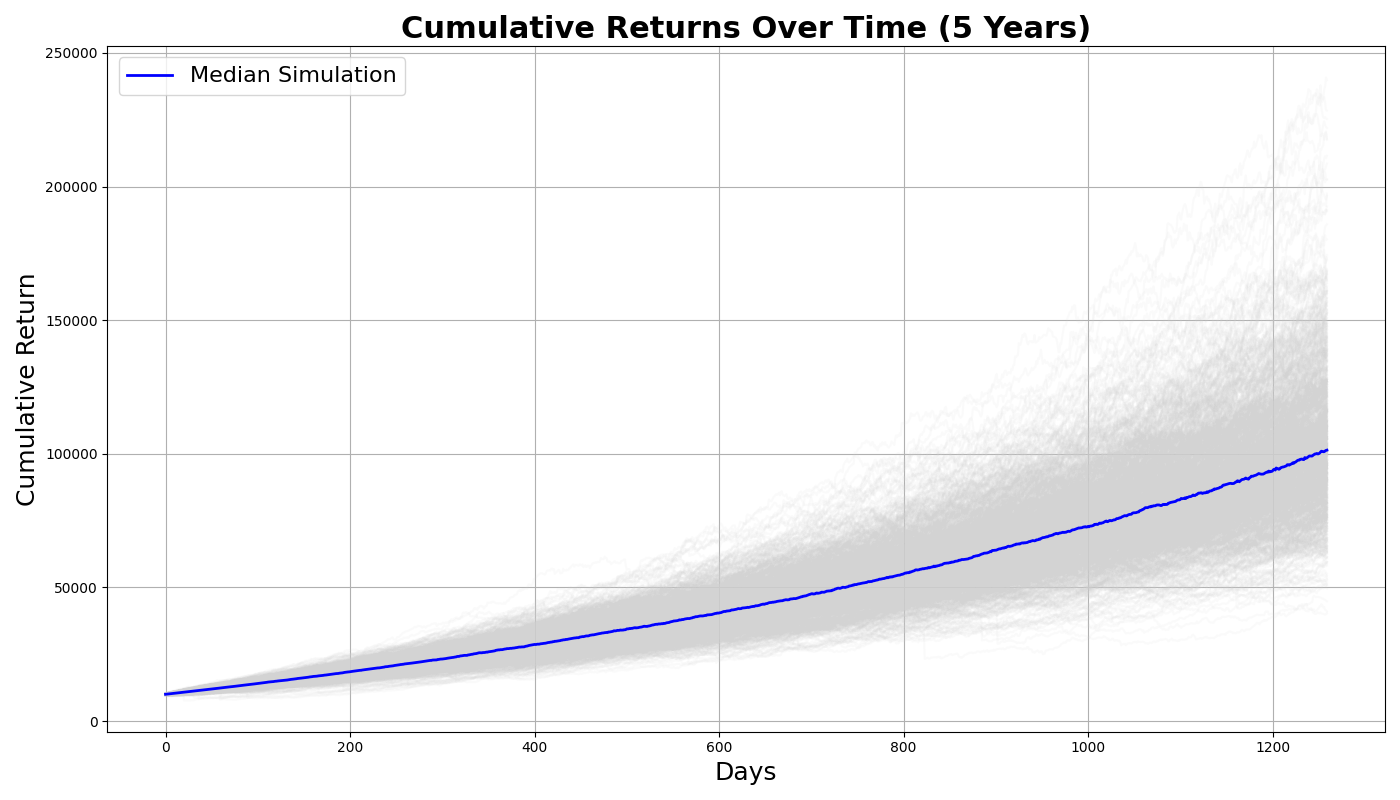
\includegraphics[width=0.8\textwidth]{../Figures/cumulative_returns_over_time_5_years.png}
    \caption{Cumulative Returns Over Time (5 Years)}
    \label{fig:cumulative_returns_5y}
\end{figure}

\begin{figure}[!htbp]
    \centering
    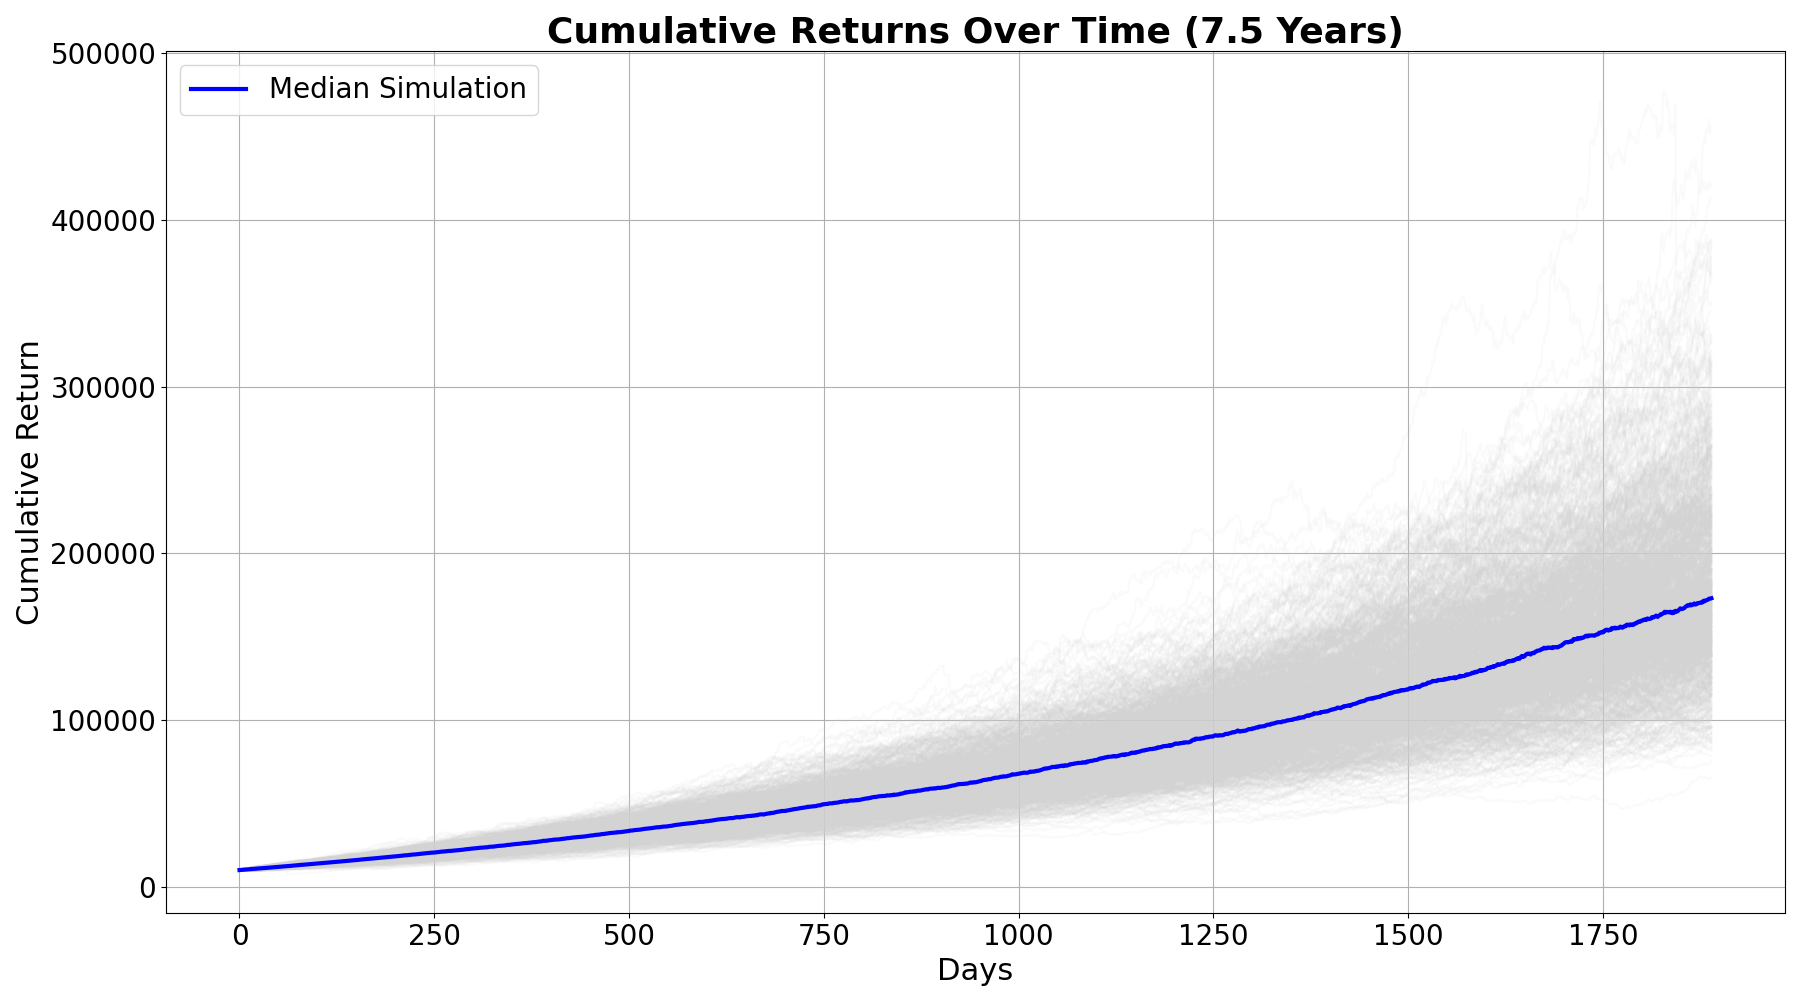
\includegraphics[width=0.8\textwidth]{../Figures/cumulative_returns_over_time_7_5_years.png}
    \caption{Cumulative Returns Over Time (7.5 Years)}
    \label{fig:cumulative_returns_7_5y}
\end{figure}

\begin{figure}[!htbp]
    \centering
    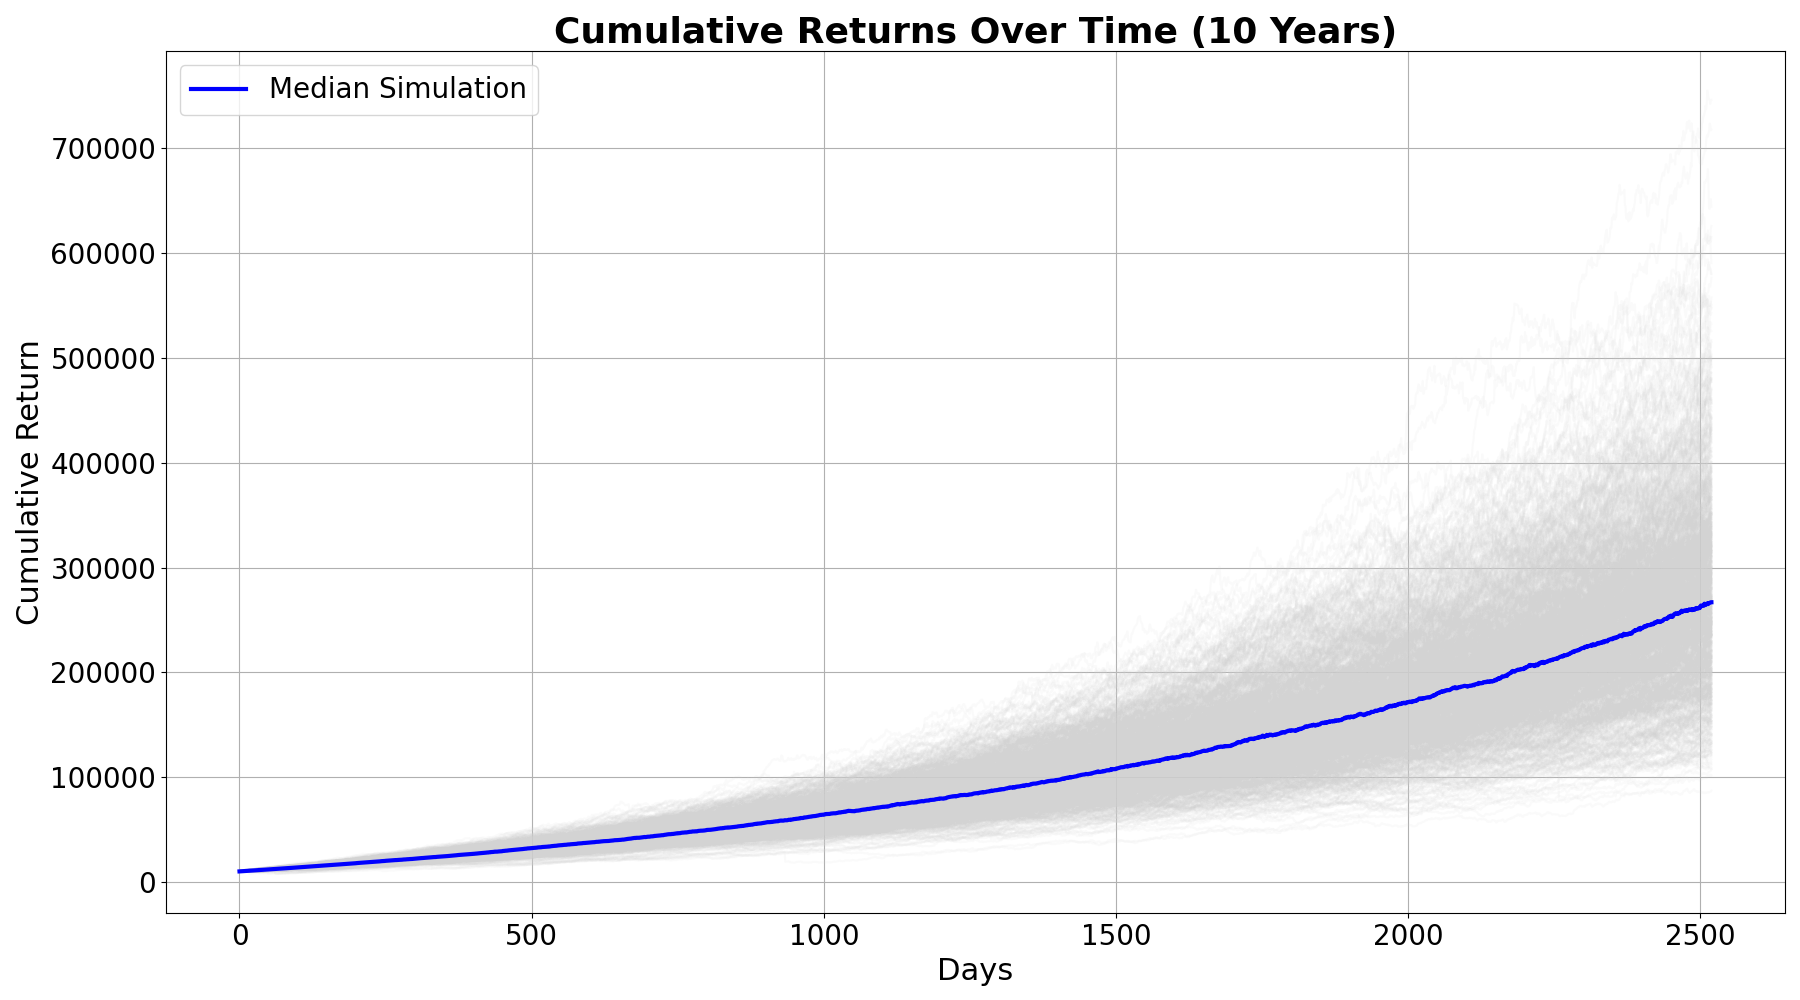
\includegraphics[width=0.8\textwidth]{../Figures/cumulative_returns_over_time_10_years.png}
    \caption{Cumulative Returns Over Time (10 Years)}
    \label{fig:cumulative_returns_10y}
\end{figure}

\textbf{Interpretation:} The Monte Carlo simulations reveal the range of possible outcomes for the portfolios over different horizons. The 5-year horizon shows greater variability, while the 10-year horizon indicates higher and more stable returns. These results underscore the benefits of long-term investment strategies \citep{glasserman2004monte}.

\subsection{Summary Statistics}
Summary statistics for the dataset are presented in Table \ref{tab:summary-stats}. These statistics were generated using the \texttt{../Data/summary\_stats.csv} file produced by the Python scripts.

\begin{table}[h!]
\centering
\scriptsize
\begin{tabular}{lccccccc}
\hline
Statistic & \begin{tabular}[c]{@{}c@{}}Mean Final \\ Portfolio Value (\$)\end{tabular} & \begin{tabular}[c]{@{}c@{}}Median Final \\ Portfolio Value (\$)\end{tabular} & \begin{tabular}[c]{@{}c@{}}10th Percentile Final \\ Portfolio Value (\$)\end{tabular} & \begin{tabular}[c]{@{}c@{}}90th Percentile Final \\ Portfolio Value (\$)\end{tabular} & \begin{tabular}[c]{@{}c@{}}Total Percentage \\ Yield (\%)\end{tabular} & \begin{tabular}[c]{@{}c@{}}Annual Percentage \\ Yield (\%)\end{tabular} \\
\hline
10-Year Horizon & 283094.44 & 265864.65 & 171232.59 & 420935.51 & 2730.94 & 39.70 \\
7.5-Year Horizon & 180745.35 & 173433.88 & 116972.91 & 256760.32 & 1707.45 & 47.10 \\
5-Year Horizon & 101559.42 & 98327.18 & 67062.20 & 139233.79 & 915.59 & 58.98 \\
\hline
\end{tabular}
\caption{Summary Statistics of the Dataset}
\label{tab:summary-stats}
\end{table}

\textbf{Interpretation:} Table \ref{tab:summary-stats} provides a detailed summary of the statistical outcomes for each investment horizon. The mean and median final portfolio values give insights into the expected performance, while the 10th and 90th percentile values offer a perspective on the range of potential outcomes. The total and annual percentage yields reflect the overall return potential of the portfolios over their respective horizons \citep{fama1970efficient}.

\newpage
